\section{Related Work}
\label{rwork}
This work relates to both hardware acceleration for LLMs and CGRA implementation.
In this section, we survey the key trends in both domains to contextualize our work and clarify its unique position and contributions.


\subsection{LLM Hardware Accelerators}
Research on hardware acceleration for LLM inference falls into three main streams. 
The primary stream centers on the use of GPGPUs.
Innovations such as Tensor Cores and the Hopper architecture\nobreak\cite{nvidia_h100} have substantially increased the throughput of LLM inference.
The high programmability and well-developed ecosystem of GPGPUs facilitate rapid prototyping and application development\cite{sze2017efficientprocessingdeepneural}.
However, this approach consumes substantial power, posing a significant sustainability challenge\cite{power_consideration}.

The second stream involves the development of ASICs specifically tailored for LLM inference. 
Architectures such as Google's TPU\nobreak\cite{TPU} and Meta's MTIA\nobreak\cite{MTIA} achieve performance and power efficiency that far surpass GPGPUs by concentrating computational resources on the large-scale dot-product operations at the core of LLMs. 
However, this high efficiency often results in over-specialization to particular algorithms or quantization methods, limiting adaptability.
Consequently, these designs inherently risk rapid obsolescence due to the difficulty in adapting to fast-evolving LLM algorithms such as Mixture of Experts~(MoE)\nobreak\cite{MoE} and Activation-aware Weight Quantization~(AWQ)\nobreak\cite{AWQ}.

The third stream, positioned between the efficiency of ASICs and the flexibility of GPGPUs, explores the use of reconfigurable hardware, such as FPGAs and CGRAs. 
These architectures have already proven effective for general AI acceleration, with numerous research demonstrating their advantages in balancing performance and power consumption~\cite{fpgacnn,li2020ftransenergyefficientaccelerationtransformers,vitisai,multi_task}. 
Based on this success, they are now emerging as a suitable solution for LLM inference. 
The reconfigurability of these devices can potentially address the inflexibility inherent in ASICs, offering a suitable approach for the rapid evolution of LLMs. 

\subsection{FPGA for LLM Inference}


Research on FPGA-based LLM acceleration is an important focus of current research in algorithm-hardware co-design\nobreak\cite{hydra,llm_agile,llm4fpga,llama2fpga}. 
For instance, UltraFormer\nobreak\cite{ultraformer} exemplifies this approach by redesigning the Transformer architecture itself for FPGAs. 
It pursues algorithmic-level optimization by integrating a linear-complexity attention mechanism with \SI[number-unit-product=\nobreakdash-]{1.58}{bit} quantization derived from BitNet\nobreak\cite{bitnet}. 
Similarly, research like BitMoD\nobreak\cite{bitmod} and AccLLM\nobreak\cite{acc_llm} have demonstrated a method for improving performance and efficiency while maintaining model accuracy. 
They achieve this by proposing custom low-bit data types, such as \SI[number-unit-product=\nobreakdash-]{2}{bit} and \SI[number-unit-product=\nobreakdash-]{3}{bit} formats, and implementing specialized arithmetic units on FPGAs to process them efficiently.

Furthermore, FPGAs provide a suitable platform for experimenting with innovative architectures to address the memory bandwidth bottleneck.
For example, FlexCiM\nobreak\cite{flex_cim} leverages fully digital compute-in-memory (DCiM) technology to support flexible structured sparsity, while MECLA\nobreak\cite{mecla} substantially reduces off-chip data transfers through a novel on-chip weight reorganization technique. 
The research area is also expanding beyond single-accelerator designs to establish development ecosystems.
A notable example is SECDA-LLM\nobreak\cite{secda-llm}, which proposes a framework for rapidly integrating FPGA accelerators within llama.cpp. 
Although FPGAs are an active area of research for LLM acceleration, they still encounter challenges such as high development complexity and inherent limitations in operating frequency and power efficiency compared to ASICs.


\begin{figure*}[t]
    \centering
    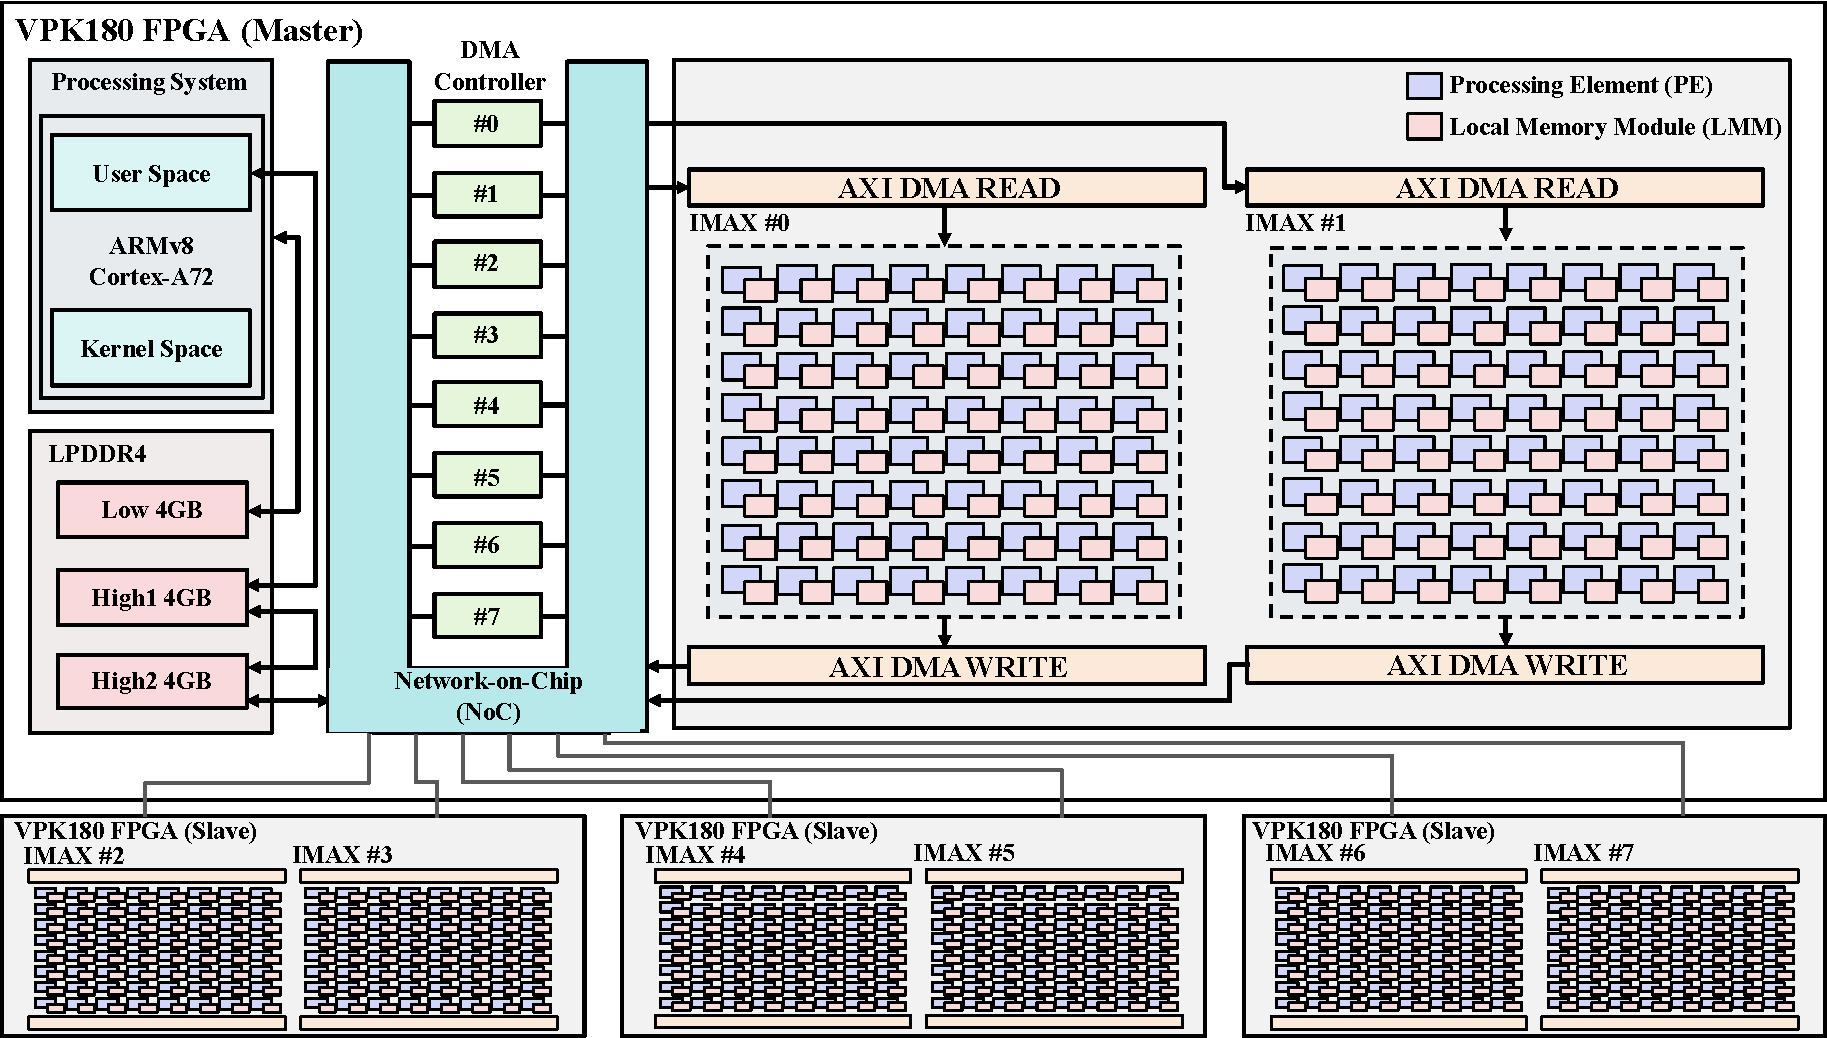
\includegraphics[width=1.95\columnwidth]{./imax3_board_config.pdf}
    \caption{ High-level overview of the IMAX3 system architecture, implemented on a multi-FPGA platform with four AMD Versal VPK180 devices.}
    \label{fig:imax3_conf}
  \end{figure*}
  
  
\subsection{CGRA for LLM Inference}
CGRAs have recently been investigated as an architectural solution to overcome the performance and programmability trade-offs of FPGAs. 
By spatially mapping dataflow graphs~(DFGs) onto an array of PEs, CGRAs achieve power efficiency approaching that of ASICs while retaining programmability through reconfiguration. 
Research on CGRAs for LLM acceleration is an emerging field, with several distinct approaches recently introduced.

Other research focuses on optimizing linear operations like Matrix-Vector Multiplication~(MVM), which represent a major computational component in LLMs. 
The CORO algorithm\nobreak\cite{coro}, for instance, exemplifies a data-centric optimization strategy, combining non-uniform quantization with variable-length data encoding. 
This technique leverages the clustering of weight values to reduce the memory footprint by encoding them in pairs. 
CORO's contribution lies in improving algorithmic memory efficiency for kernel-level performance on flexible accelerators. 
However, it does not extend to broader architectural and system-level challenges.

Another research direction focuses on the optimization of non-linear operations. 
While these operations account for a smaller portion of the total computation compared to MVM, they often become significant latency bottlenecks. 
A representative work in this area is PICACHU\nobreak\cite{picachu}, a plug-in CGRA accelerator designed to efficiently handle diverse non-linear functions such as Softmax and normalization. 
It is designed to complement existing LLM accelerators by offloading only non-linear computations to the CGRA.


Our work differs from these works in two key aspects: its architectural philosophy and its evaluation methodology. 
First, regarding our architectural philosophy, we emphasize architectural versatility. 
Similar to CORO, our work focuses on offloading dot-product operations, which account for the majority of the computational load in LLMs. 
In contrast to CORO, which is designed specifically for dot-product operations in LLMs, our IMAX architecture is a general-purpose CGRA that is not limited to a single task or model.
We have already demonstrated its capability on diverse workloads such as FFT\nobreak\cite{imax3} and CNNs\nobreak\cite{cnn_imax_1,cnn_imax_2}.
This research shows that the same architecture can achieve high energy efficiency on modern LLM inference tasks without modification, demonstrating a design principle for sustainable hardware that avoids task-specific specialization.
A second key difference is our evaluation methodology. 
We assess E2E system performance using the widely used llama.cpp framework. 
This approach enables the assessment of E2E system performance under realistic conditions. 
Our analysis incorporates important factors such as host-CPU interaction, DMA transfer overheads, and complex software control. 
In the emerging field of LLM acceleration on CGRAs, this paper provides a comprehensive characterization of the performance and challenges of a versatile architecture at a full-system level.




While a direct quantitative comparison with other FPGA and ASIC-based LLM accelerators is valuable, achieving a fair comparison is challenging.
This is due to discrepancies in target models, quantization schemes, process technologies, and evaluation methodologies.
For instance, some studies use isolated kernel benchmarks, whereas others perform E2E system-level measurements.
Many papers report performance in TOPS or TOPS/W based on peak theoretical throughput, figures that often omit significant system-level overheads.
Therefore, this work provides a detailed performance analysis of a general-purpose, non-specialized CGRA architecture, using the industry-standard llama.cpp. 
The C++ framework is used unmodified, and we compare our results against those of GPU platforms. 
Our evaluation inherently incorporates host-accelerator interactions and data transfer overheads, thereby offering a realistic assessment of system-level performance and energy efficiency.


  

  
%   \begin{figure}[t]
%     \centering
%     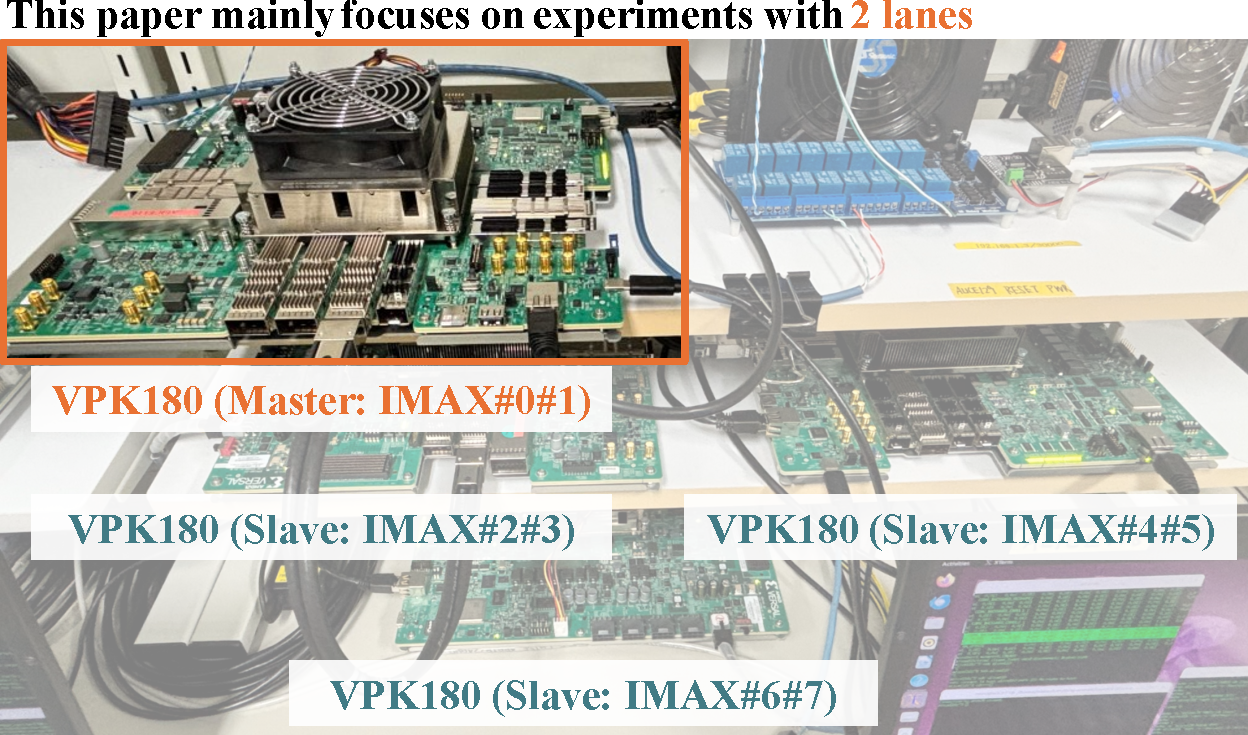
\includegraphics[width=0.9\columnwidth]{./imax3_proto.pdf}
%     \caption{IMAX3 prototype board}
%     \label{fig:imax3_proto}
%   \end{figure}
  

\subsection{CGLA architecture and IMAX}
The IMAX architecture is based on a different design approach from those previously mentioned.
The architecture is designed for task-agnostic versatility, providing both linear scalability and high programmability through direct compilation from C/C++.
IMAX employs a CGLA structure, arranges PEs and LMMs in an alternating pattern in a one-dimensional array. 
This design addresses the complex routing and compilation challenges of conventional 2D mesh-based CGRAs.
The combination of this simple structure with multi-functional, CISC-based PEs allow IMAX to efficiently execute diverse workloads. 
These include not only linear operations like General Matrix Multiplication~(GEMM) but also those involving irregular memory accesses and complex control flows.
This linear topology is particularly well-suited for the dot-product operations that dominate LLM inference, providing a theoretical basis for its high energy efficiency. 
Specifically, weights and activations can be streamed through the one-dimensional array of PEs, creating a deep, deterministic pipeline. 
This structure improves spatial data locality and reuse. 
Data passed from one PE is immediately consumed by its neighbor, which eliminates the need for complex routing or access to a higher-level memory hierarchy.
The highly regular and predictable memory access patterns inherent in this dataflow execution minimize the energy overhead associated with data movement and address calculation. 
These factors contribute significantly to reducing power consumption in conventional architectures.


\begin{figure}[t]
    \centering
    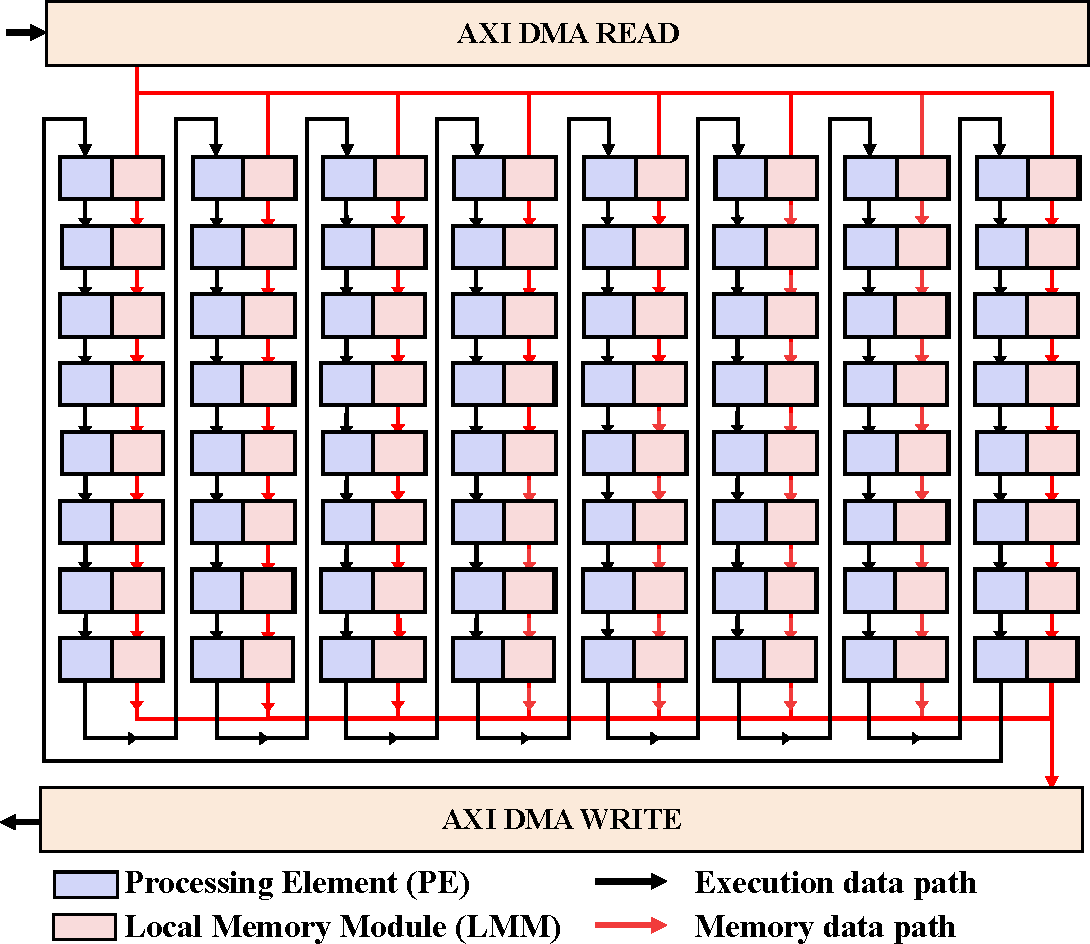
\includegraphics[width=0.95\columnwidth]{./pe_detailed.pdf}
    \caption{ Inter-PE and LMM connections within a single IMAX compute lane.}
    \label{fig:pe_detailed}
\end{figure}


Fig.~\ref{fig:imax3_conf} provides a high-level overview of the IMAX3 system architecture. 
Implemented on an AMD Versal VPK180 FPGA, IMAX3 is a System-on-Chip~(SoC) consisting of a Processing System~(PS) and Programmable Logic~(PL). 
The PS serves as the host, featuring a dual-core Arm Cortex-A72 processor running Linux. 
It manages the entire workflow, from application compilation to execution control. 
A high-bandwidth Network-on-Chip~(NoC) facilitates communication between the PS and PL, while a dedicated DMA controller efficiently transfers data between system memory and the accelerator.
The accelerator core itself resides within the PL. 
It consists of eight independent compute lanes. 
This multi-lane design is central to the architecture's scalability, as performance can be tailored by allocating a variable number of lanes to match an application's degree of parallelism.



The internal structure of each compute lane is depicted in Fig.~\ref{fig:pe_detailed}. 
This illustrates the core CGLA structure of IMAX, where PEs and LMMs are arranged alternately in a one-dimensional array. 
This linear topology simplifies the data paths between PEs, facilitating easier compilation while also enabling low-latency access to adjacent LMMs. 
Data is loaded into the LMMs via DMA and then forms a pipelined dataflow across the PEs, which is essential for maintaining high utilization of the arithmetic units.

Fig.~\ref{fig:execution_unit} details the internal architecture of an individual PE. 
Each PE features a heterogeneous design, comprising multiple arithmetic units, address generation units, and LMMs. 
The arithmetic component consists of three ALUs (ALU1, ALU2, and ALU3), dedicated to integer, logical, and shift operations, respectively, which enables the parallel execution of diverse instructions. 
The Address Generation Units (AG1, AG2) operate independently of the ALUs to calculate memory addresses. 
This design decouples the computation and memory access pipelines, thereby improving execution efficiency. 
The LMM is implemented with a hardware-managed double-buffered configuration, a key feature designed to enable the concurrent execution of computation and data transfers. 
While one buffer is being used by the PEs for active computation, the DMA controller can simultaneously load the next set of data into the other buffer. 
This mechanism is intended to mask memory access latency by overlapping communication with computation, thereby maximizing data throughput.
The integration of these components allows each PE to efficiently process the large volumes of data demanded by high-performance computing tasks.

Previous work has established IMAX3 as a general-purpose computing platform. 
Its effectiveness has been demonstrated across a wide spectrum of workloads. 
These range from traditional kernels, such as SpGEMM, FFT\nobreak\cite{imax3}, light-field image processing\nobreak\cite{light_field_imax} to modern AI applications such as CNNs\nobreak\cite{cnn_imax_1,cnn_imax_2}, Graph Convolutional Networks~(GCNs)\nobreak\cite{gat_imax}, and Retrieval-Augmented Generation (RAG) systems\nobreak\cite{knn_imax}.
This work applies these findings to the domain of LLMs. 
Our previous works\nobreak\cite{first_llm_imax,llama2_imax} presented the implementation of a Llama2-based model on IMAX, confirming its feasibility.
Based on that success, this work aims to validate the performance and robustness of IMAX as an LLM accelerator using a wider range of models and workloads.
To validate the generalizability of the architecture, we evaluate its robustness against the Qwen3 family, which features diverse model structures.
Therefore, we expand our evaluation to the state-of-the-art Qwen3 family to assess its practical performance.


\begin{figure}[t]
    \centering
      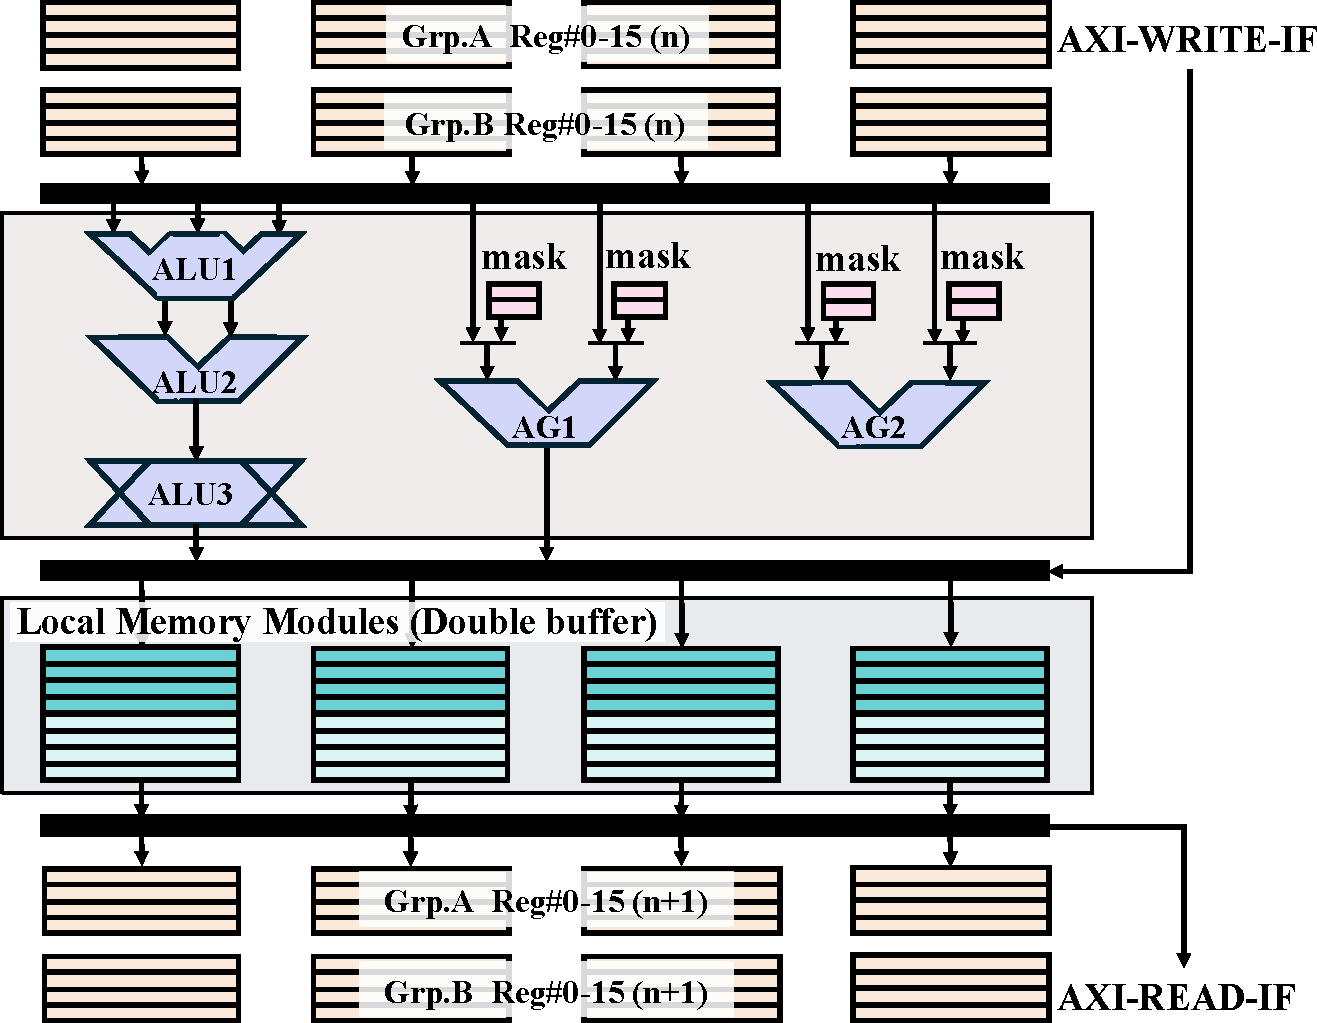
\includegraphics[width=0.95\columnwidth]{./internal_pe.pdf}
    \caption{Detailed architecture of a single IMAX PE.}
    \label{fig:execution_unit}
  \end{figure}

